% !TeX root = ../main.tex
\chapter{ROS与半实物仿真}
本章分为ROS(robot operating system)下的软件在环仿真、半实物的硬件在环仿真以及软件在环仿真下的offboard轨迹跟踪对比实验。

软件在环仿真(SITL,software in the loop),软件是基于PX4固件改动其运动控制部分的代码后编译而来的。仿真在ROS+gazebo环境中进行,支持运行offboard控制程序,使无人机跟踪指定轨迹。

硬件在环仿真(HITL,hardware in the loop),将上一阶段修改后的PX4固件烧写到pixhawk飞控板中,使得控制器从仿真变为实物(也是后续实机实验的真实控制器)。接入gazebo仿真环境,验证固件在飞控板的nuttx实时操作系统中能否正常运行。但需要说明的是,HITL并不支持接入ROS,那么也就不能进行offboard控制,这一步只能通过仿真动画做定性验证。

offboard轨迹跟踪实验在软件在环仿真下进行,通过offboard控制程序向无人机发布一连串的期待位置,与PX4原生固件对比控制效果。

ROS框架下的仿真实验,控制器和被控对象都会更贴近现实,会有来自传感器的噪声等影响,控制器的控制周期也不再是Matlab中理想的同步固定周期,而是要依赖多个异步异周期的反馈信号,还会受到计算速度波动的影响。

\section{软件在环仿真}
Matlab仿真只是初步验证了HOFA方法的有效性,既没有考虑实际的飞控固件中异步的采样周期、进程管理等因素,也没有考虑内部和外部传感器信息融合的因素。而在ROS+gazebo下的软件在环仿真会考虑以上因素,进一步贴近实际情况。

\subsection{环境配置}
由于当前ros2适配的各种依赖库包括PX4的版本都还在不停迭代,因此目前还是选择更为稳定、资料更多的ros1。在ubuntu20.04中安装ros1 noetic以及配套的gazebo11 classic(使用鱼香ros一键安装\cite{fishros}时会同步安装),然后从GitHub上clone最近的发行版PX4 v1.14.0,注意要使用递归将所有子项目克隆下来。
\begin{lstlisting}[language=Bash, basicstyle=\footnotesize, linewidth=\linewidth]
  git clone -b v1.14.0 https://github.com/PX4/PX4-Autopilot.git --recursive
\end{lstlisting}

然后运行以下命令以解决依赖。

\begin{lstlisting}[language=Bash, basicstyle=\footnotesize, linewidth=\linewidth]
  Bash Tools/setup/ubuntu.sh
\end{lstlisting}

最后运行软件在环仿真命令:

\begin{lstlisting}[language=Bash, basicstyle=\footnotesize, linewidth=\linewidth]
  make px4_sitl gazebo-classic
\end{lstlisting}

运行成功后会进入gazebo仿真界面,打开QGC会自动连接地面站,在地面站中可以方便地看到回传的位姿信息并且发布起飞和指点飞行命令,如图 \ref{sitl}。在使用gazebo仿真时,需要安装显卡驱动,否则画面渲染将完全使用CPU,这会导致严重的卡顿。

\begin{figure}[h]
  \centering
     \begin{minipage}[c]{0.45\textwidth}
      \centering
      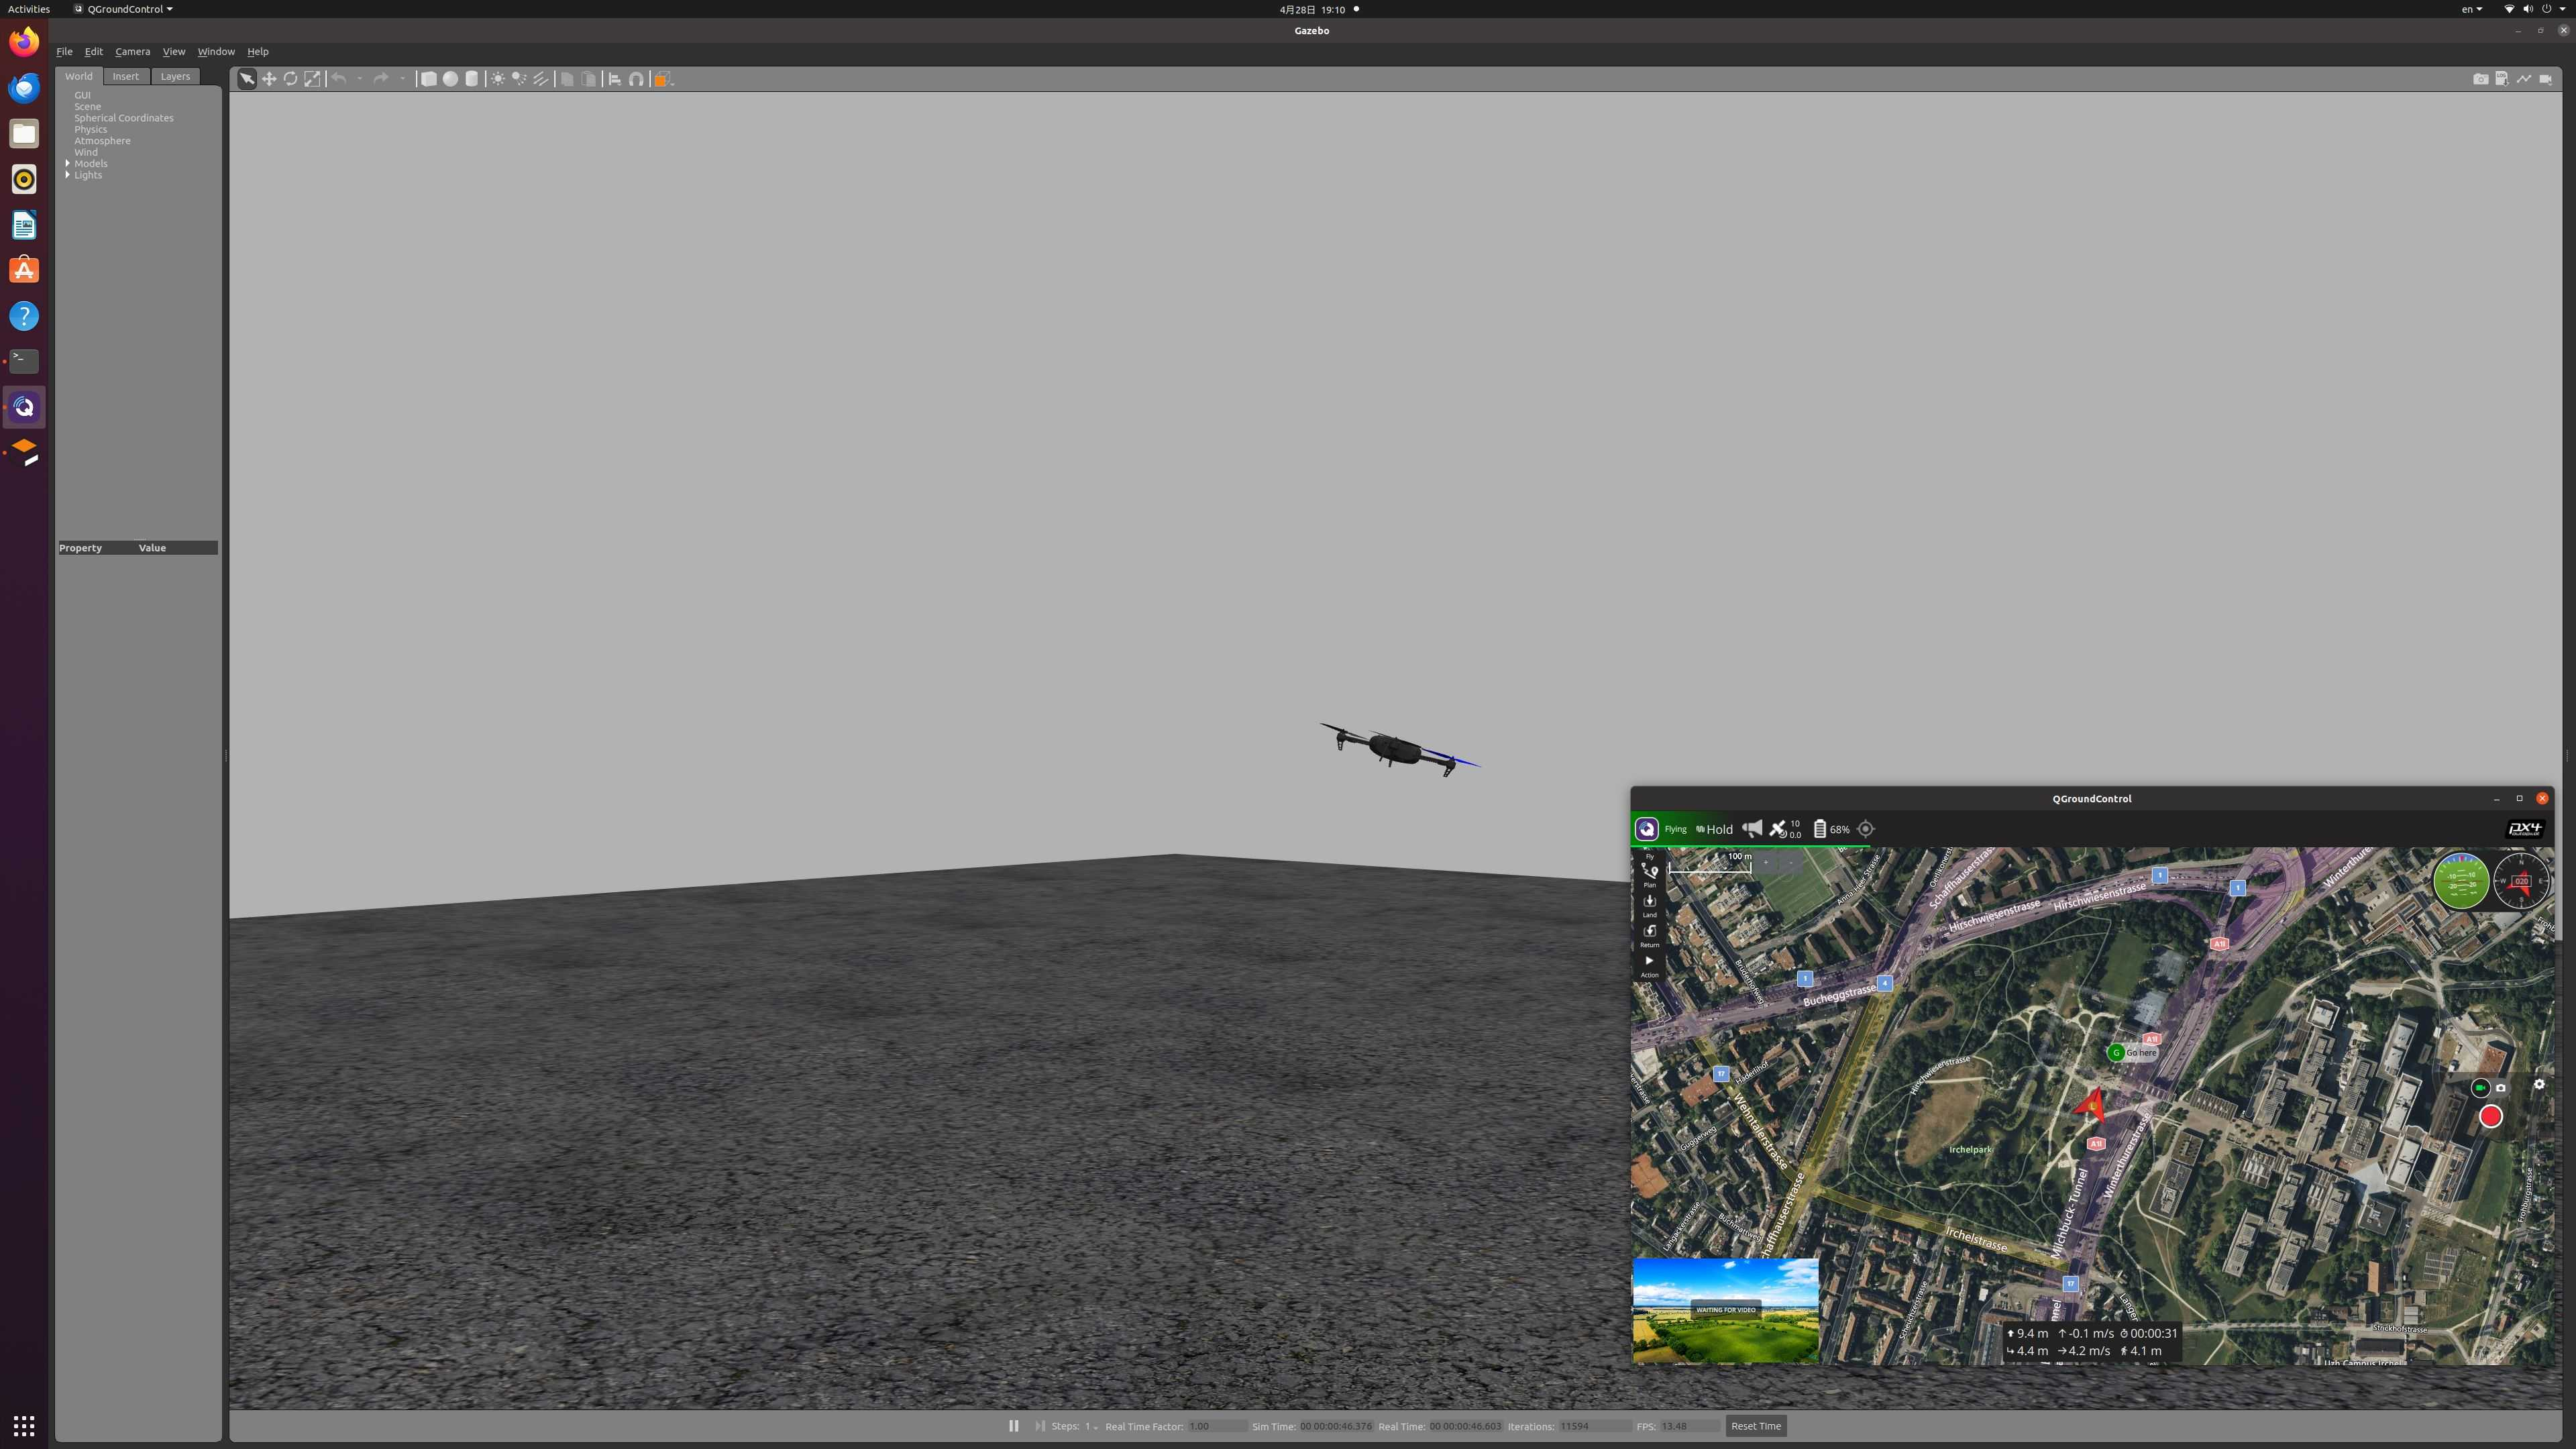
\includegraphics[width=0.9\textwidth]{sitl1.png}
   \end{minipage}%
     \begin{minipage}[c]{0.45\textwidth}
      \centering
      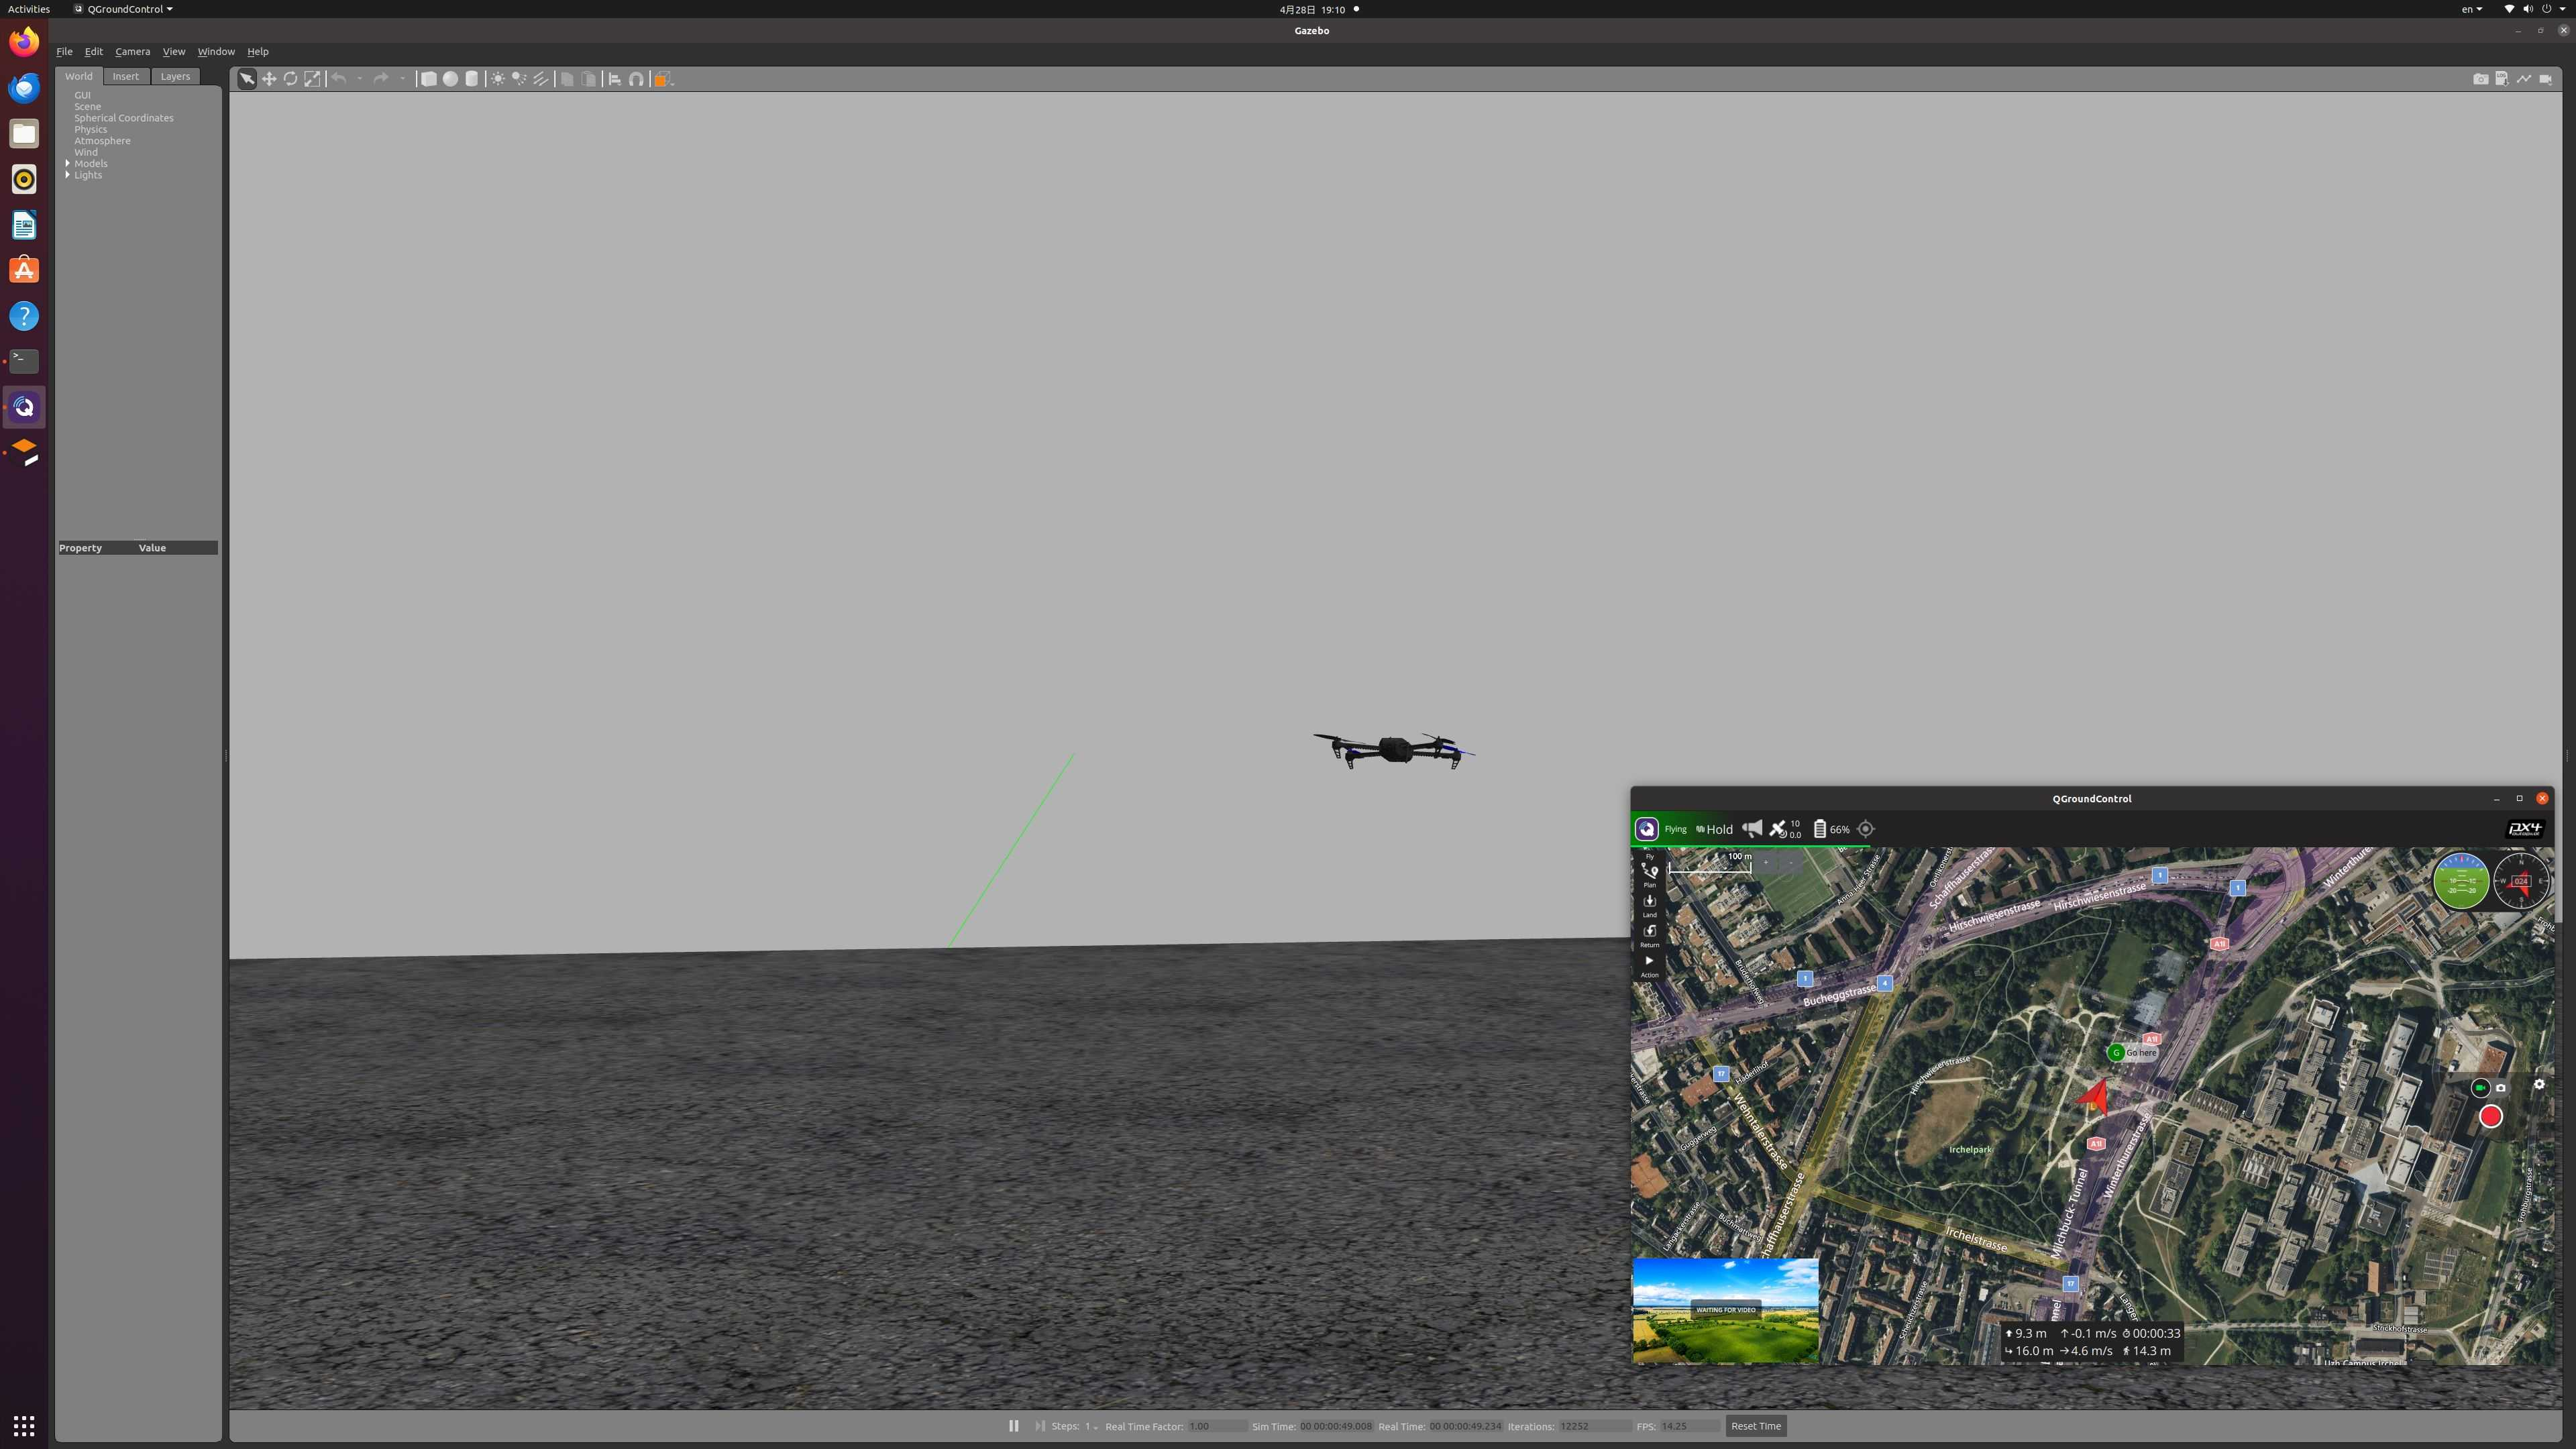
\includegraphics[width=0.9\textwidth]{sitl2.png}
   \end{minipage}
   \caption{SITL gazebo界面以及QGC指点控制}
   \label{sitl}
 \end{figure}

 这里默认使用的是内置的iris无人机模型,有关该模型的具体参数可以在源码\cite{iris}中查到:
 \begin{lstlisting}[language=Bash, basicstyle=\footnotesize, linewidth=\linewidth]
  <inertial>
    <pose>0 0 0 0 0 0</pose>
    <mass>1.5</mass>
    <inertia>
      <ixx>0.029125</ixx>
      <ixy>0</ixy>
      <ixz>0</ixz>
      <iyy>0.029125</iyy>
      <iyz>0</iyz>
      <izz>0.055225</izz>
    </inertia>
  </inertial>

...

<box>
  <size>0.47 0.47 0.11</size>
</box>
 \end{lstlisting}
 
由于SDF文件的特殊性,不建议修改iris模型参数去匹配控制器中的设定,而是修改控制算法中的参数来匹配iris模型。HOFA算法对于转动惯量参数有一定鲁棒性,但如果有数量级的差距还是会导致严重问题。

其实到此为止只完成了gazebo下的仿真,并没有接入ros的框架,也就无法使用rostopic等命令进行进一步调试。接入ros框架还需要运行以下命令:

\begin{lstlisting}[language=Bash, basicstyle=\footnotesize, linewidth=\linewidth, breaklines=true]
  sudo apt-get install ros-noetic-mavros ros-noetic-mavros-extras

  wget https://raw.githubusercontent.com/mavlink/mavros/master/mavros/scripts/install_geographiclib_datasets.sh
  bash install_geographiclib_datasets.sh

  cd PX4-Autopilot
  make px4_sitl_default gazebo
\end{lstlisting}

安装mavros包并运行官方的bash文件解决依赖;重新编译SITL固件(命令与gazebo中有细微差别,但生成的build文件名相同)。

  \begin{lstlisting}[language=Bash, basicstyle=\footnotesize, linewidth=\linewidth, breaklines=true]
  source Tools/simulation/gazebo-classic/setup_gazebo.bash $(pwd) $(pwd)/build/px4_sitl_default
  export ROS_PACKAGE_PATH=$ROS_PACKAGE_PATH:$(pwd)
  export ROS_PACKAGE_PATH=$ROS_PACKAGE_PATH:$(pwd)/Tools/simulation/gazebo-classic/sitl_gazebo-classic

  roslaunch px4 mavros_posix_sitl.launch
\end{lstlisting}

在每一次打开新终端后都需要执行:配置ros环境变量使roslaunch能找到PX4包内的文件;launch文件中包含了仿真的各种可调节参数,包括gazebo环境和初始位置等。

运行后可以用rqt\_graph命令看到节点和消息,如图\ref{sitlrqt}所示。mavros将整个飞控虚拟化为一个节点,我们可以通过mavlink stream命令修改imu等数据发布的频率。但是,这不是飞控内部的控制频率,仅仅是通过mavros向外部发送信息的频率。所以,无法直接用该命令改变控制周期。
\begin{figure}[!h]
  \centering
  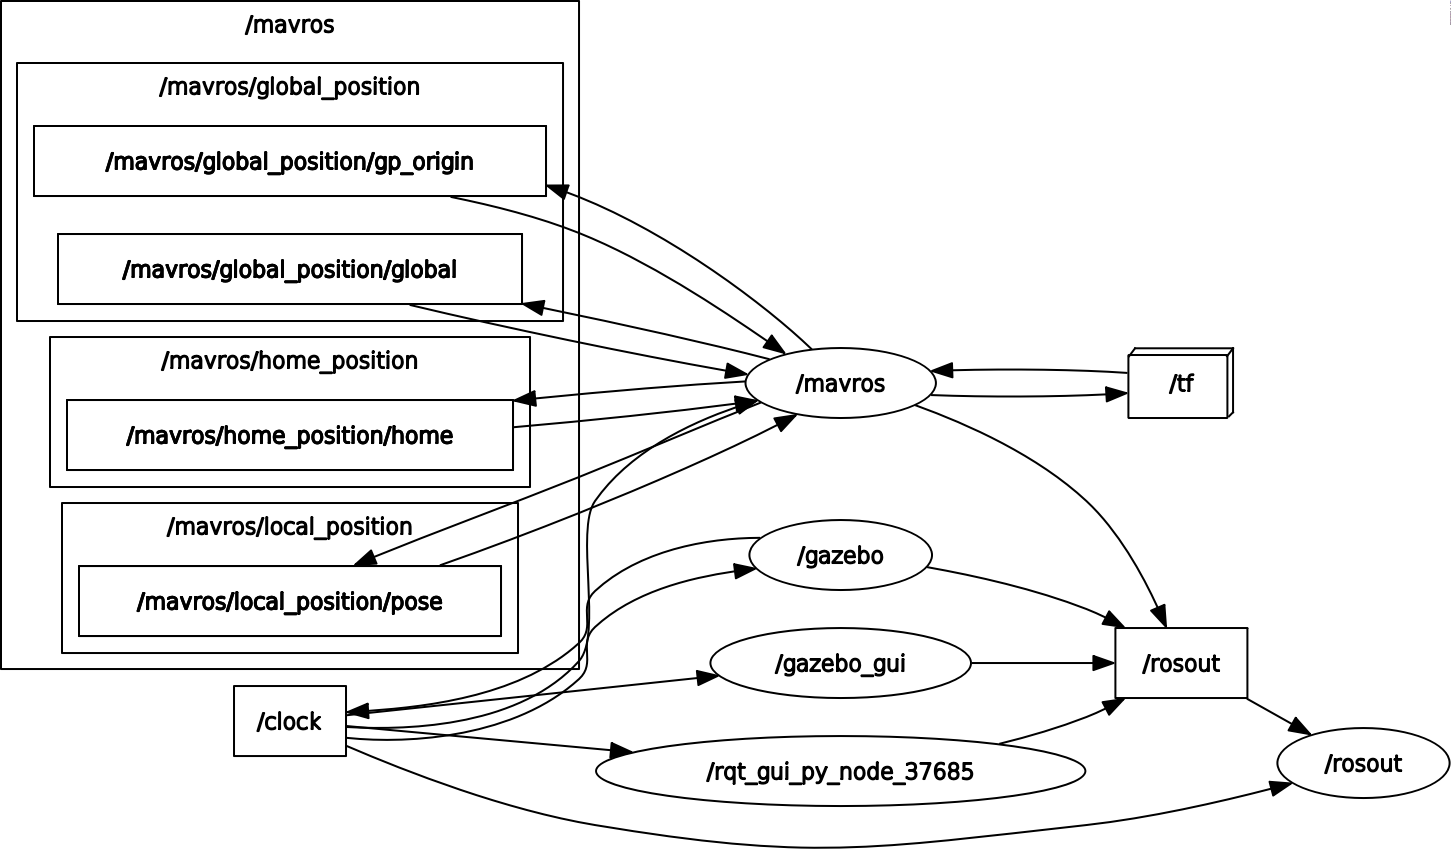
\includegraphics[width=0.6\textwidth]{sitlrqt.png}
  \caption{软件在环仿真ros节点和话题示意图}
  \label{sitlrqt}
\end{figure}

 \subsection{HOFA算法植入}
在环境配置完成后,接下来就要在PX4源码的基础上修改多旋翼运动控制部分的代码,将其原本的“位置-速度-角度-角速度”四环PID控制 \cite{px4控制}改为HOFA控制。

PX4是一个适用于固定翼、直升机、四旋翼、地面车辆乃至于船舶等多种形式机器人的自动驾驶仪,既可以进行软件仿真,也能将固件烧写到硬件中进行实机实验,其架构十分复杂。在多旋翼部分中,就包含多渠道的传感器信息订阅和融合、多个节点间信息的传递,支持实时在地面站修改各种控制参数,支持包含自稳、高度、位置和offboard等多种飞行模式。因此PX4拥有庞大的规模和错综复杂的上层架构,因此在算法植入时,我们将尽可能不改动上层架构,在相应的包内尽量保持输入输出接口不变,避免引起未知的错误。

PX4运行在嵌入式系统上,通常使用Nuttx操作系统,这是一个实时操作系统(RTOS),专为微控制器设计。由于不同类型的传感器采样周期不同,不同环节的控制器周期也不同,PX4采用异步的线程管理方法以尽量减少时延。传感器采样并处理得到估计后,标记更新,轮询的控制器进程判断数据已经更新过,就进入控制,发布新的控制量到下一环节:姿态环在姿态更新后控制,位置环在位置更新后控制。因此控制频率的上限取决于传感器的采样频率,设定值(setpoint)的更新频率不会制约控制频率,在下一个设定值更新前,将沿用之前的设定值。

\textbf{位置环}

如理论设计一章末尾所提到的,PX4原本的位置环不需要做任何更改,只需要在地面站中调节相应的参数数值就能实现我提出的位置环控制方法。以下对位置环软件包做简单介绍:

PX4的多旋翼位置环控制位于src/modules/mc\_pos\_control包中,包内层次结构如图\ref{mc_pos}。MulticopterPositionControl.cpp和MulticopterPositionControl.hpp主要负责与外部的消息传递,用其Run()函数启动一个位置环(包括位置和速度)控制的进程,其真正的控制代码在mc\_pos\_control/PositionControl/PositionControl.cpp以及其对应的头文件中。

\begin{figure}[!h]
  \centering
  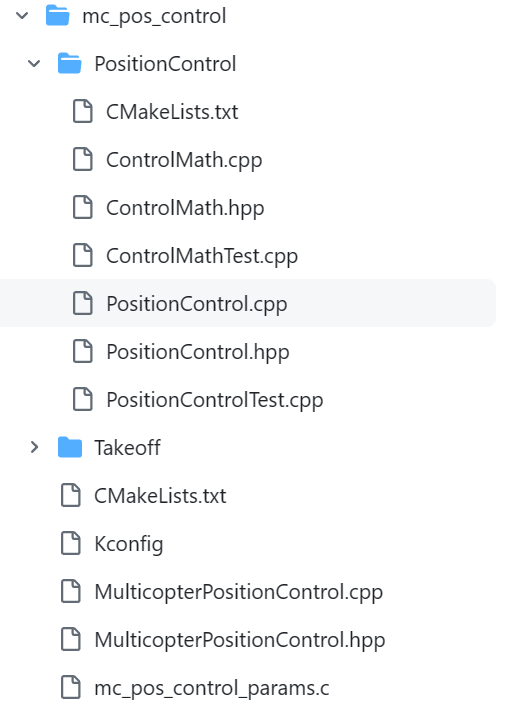
\includegraphics[width=0.3\textwidth]{mc_pos.png}
  \caption{mc\_pos\_control包结构}
  \label{mc_pos}
\end{figure}

而位置和速度的控制律,也就是LQR解算得到的K(只在对角线有非零值),可以借MPC\_XY\_P、MPC\_Z\_P、MPC\_XY\_VEL\_P\_ACC、MPC\_Z\_VEL\_P\_ACC这四个参数作为变量载体。由于实机的前后和左右也基本对称,xy轴可以使用同样的参数。可以在地面站对这些参数进行实时的调整。

位置环的输出除了期望的推力矢量,还有根据期望推力矢量和期望偏航角生成的期望姿态,这部分函数在ControlMath.cpp中。PX4这部分算法的逻辑与HOFA中的完全一致。

\textbf{姿态环}

PX4的多旋翼姿态环控制分别在mc\_att\_control和mc\_rate\_control两个包内,两者间通信的管道是mc\_att\_control向mc\_rate\_control发布期望的角速度“rate\_setpoint”,为了尽量不更改架构,我们接下来也将沿用这一通信管道。

原本的控制算法不需要前一时刻的期望姿态,因此首先要在AttitudeControl.hpp中定义新的变量,包括前一时刻的期望姿态,以及期望姿态生成时的时间(包含在期望姿态结构体中)。原本的mc\_att\_control不需要角速度信息,因此需要额外添加uORB::SubscriptionCallbackWorkItem函数订阅角速度信息。

然后在AttitudeControl.cpp中植入HOFA的核心部分。四元数和旋转矩阵的运算函数在namespace matrix下已有定义。$R$和$R_d$的更新频率并不相同,$R$的更新频率取决于imu等传感器的估计值的发布频率,$R_d$的更新频率取决于位置环产生期望姿态的频率。$R$的更新频率要高于$R_d$,也就是说,前后多个控制周期内,控制计算会根据同一个$R_d$和不同的$R$进行。误差向量$e$的导数估计会根据前后两个$e$的差分除以$R$的更新周期来近似。

最终将计算得出的除了$\omega \times J\omega$的期望力矩通过“rate\_setpoint”的传输通道,传递给mc\_rate\_control。无人机的转动惯量参数和姿态控制律的具体数字,直接在AttitudeControl.cpp中定义。如果后续需要调试,则要在源码上进行修改。

进一步在mc\_rate\_control阅读代码,发现包内的MulticopterRateControl.cpp主要做了线程管理和消息更新的工作,真正的控制算法在其Run()函数中调用的RateControl::update()中,这个类函数位于src/lib/rate\_control/rate\_control.cpp。然后就在这个函数中略加修改,完成整个HOFA算法的植入。

\textbf{总结}

总共在五个代码文件中做了修改,分别是:
\begin{itemize}
 % \item src/modules/mc\_pos\_control/PositionControl/PositionControl.cpp
  \item src/modules/mc\_att\_control/mc\_att\_control\_main.cpp
  \item src/modules/mc\_att\_control/mc\_att\_control.hpp
  \item src/modules/mc\_att\_control/AttitudeControl/AttitudeControl.hpp
  \item src/modules/mc\_att\_control/AttitudeControl/AttitudeControl.cpp
  \item src/lib/rate\_control/rate\_control.cpp
\end{itemize}

用修改过的这五个文件替换先前环境配置环节中编译完成的包中对应的文件(由于用于修改的代码文件下载时没有递归下载子项目,无法直接编译,且在原本已经过编译的文件夹上修改会更稳妥),再运行make px4\_sitl\_default gazebo命令即可,效果与图\ref{sitl} 基本相同。两种控制方法的定量对比会在实机实验时展开,此处只是粗略验证可行性。

\section{硬件在环仿真}
硬件在环仿真的主要目的在于,在gazebo仿真环境中初步测试生成的固件代码,防止直接进行实机实验可能出现的破坏性故障。硬件在环仿真也要首先配置环境,用PX4的发行版跑通流程;然后向飞控刷入植入HOFA的固件,进行硬件在环仿真。

\textbf{环境配置}

硬件在环仿真在软件在环仿真已经跑通的基础上并不困难,PX4的官方文档也提供了相对全面的流程\cite{px4hitl}。

首先用USB连上飞控,在QGC中进行设置:机架选择HITL兼容的Generic Quadcopter,重启;使能HITL;在应用设置中的自动连接选项,仅选择UDP(这一步做完后,直接用USB连接飞控将无法自动连入地面站)。以上步骤做完后,断开飞控连接并关闭地面站。

然后是在PX4\_Autopilot包内做软件上的配置\cite{px4hitl}:

确保QGC关闭的情况下,编译并且不运行仿真固件:
\begin{lstlisting}[language=Bash, basicstyle=\footnotesize, linewidth=\linewidth, breaklines=true]
  cd <Firmware_clone>
  DONT_RUN=1 make px4_sitl_default gazebo-classic
\end{lstlisting}

打开模型的sdf文件:

Tools/simulation/gazebo-classic/sitl\_gazebo-classic/models/iris\_hitl/iris\_hitl.sdf

找到文件的mavlink\_interface plugin分区,将 serialEnabled 和 hil\_mode 参数更改为 true。

接下来是在每个新的终端中都要执行的命令:

\begin{lstlisting}[language=Bash, basicstyle=\footnotesize, linewidth=\linewidth, breaklines=true]
  cd PX4_Autopilot
  source Tools/simulation/gazebo-classic/setup_gazebo.bash $(pwd) $(pwd)/build/px4_sitl_default
  gazebo Tools/simulation/gazebo-classic/sitl_gazebo-classic/worlds/hitl_iris.world
\end{lstlisting}


需要注意的是,在最后一步run gazebo时,飞控需要已经通过USB连在电脑上。然后打开QGC,即可进行起飞和指点飞行,如图\ref{hitl}所示。
\begin{figure}[!h]
  \centering
  \includegraphics[width=0.6\textwidth]{hitl.jpg}
  \caption{硬件在环仿真示意图}
  \label{hitl}
\end{figure}

在飞控接有遥控接收机时,也可以使用遥控器对gazebo中的虚拟飞机进行操控。

\textbf{固件烧写}

在环境配置完成后,将HOFA版本的固件编译并烧写进飞控硬件中,只需要执行以下命令:

\begin{lstlisting}[language=Bash, basicstyle=\footnotesize, linewidth=\linewidth, breaklines=true]
  cd PX4_Autopilot
  make px4_fmu-v6c_default
  make px4_fmu-v6c_default upload
\end{lstlisting}

接下来运行gazebo即可完成HOFA算法的硬件在环仿真。从仿真视频来看,控制效果良好。接下来要进入Offboard模式,用mavros发布“8”字型轨迹,分析飞行日志得到量化的结果。

\section{Offboard控制}

在PX4中,Offboard控制模式是一种允许无人机通过外部计算设备进行控制的飞行模式,而非常规的遥控器。在Offboard模式下,无人机的所有飞行控制决策(如起飞、降落、航向、速度和姿态调整)可以通过MAVLink协议从外部计算设备发送指令来实现。因而,可以在Offboard模式下任意指定无人机要跟踪的轨迹。

由于SITL是在ROS框架下,只需要编写一个Offboard控制的软件包即可通过mavros发布位置指令。

\begin{lstlisting}[language=Bash, basicstyle=\footnotesize, linewidth=\linewidth, breaklines=true]
  mkdir -p offboard_ws/src
  cd offboard_ws/src

  catkin_create_pkg offboard_run roscpp std_msgs geometry_msgs mavros_msgs
  
  cd offboard_run/src
  gedit offboard_run_node.cpp
\end{lstlisting}

该文件就是Offboard控制的核心,PX4官网提供了基础的样例\cite{Offboard}。该样例的功能是使无人机悬停在$2m$的空中,在其基础上修改,使无人机跟踪“8”字型轨迹。由于该文件要在后续实机实验中复用,而实验场地的空间有限,轨迹相较于Matlab中的做了等比缩小处理,高度也固定在$1.2m$。

保存更改后在CMakeLists.txt中加入编译指向,并编译工作空间。

\begin{lstlisting}[language=Bash, basicstyle=\footnotesize, linewidth=\linewidth, breaklines=true]
  cd offboard_run
  gedit CMakeLists.txt
  
  add_executable(${PROJECT_NAME}_node src/offboard_run_node.cpp)
  target_link_libraries(${PROJECT_NAME}_node    ${catkin_LIBRARIES})
  
  cd ~/Desktop/offboard_ws
  catkin_make
\end{lstlisting}
  
Offboard包配置完成,后续无论是SITL、HITL还是实机实验,只要在mavros节点打开的情况下,就可以用以下命令运行Offboard控制,使无人机跟踪“8”字型轨迹。

\begin{lstlisting}[language=Bash, basicstyle=\footnotesize, linewidth=\linewidth, breaklines=true]
  cd ~/Desktop/offboard_ws
  source ./devel/setup.bash
  rosrun offboard_run offboard_run_node
\end{lstlisting}

轨迹跟踪的控制效果可以从飞行日志记录的原始数据中得到。通过QGC下载.ulog文件,有多种方式可以直接可视化地查看飞行数据,如在线的Flight Review、本地的PlotJuggler等,都能直观快捷地看到大量数据曲线。

为了能够定量地分析轨迹跟踪的效果,用ulog2csv命令将飞行日志转成csv文件,提取其中位置和期望位置的文件,在Matlab中绘图和分析。

\begin{figure}[htb]
  \centering
  \begin{minipage}[b]{0.49\linewidth}
      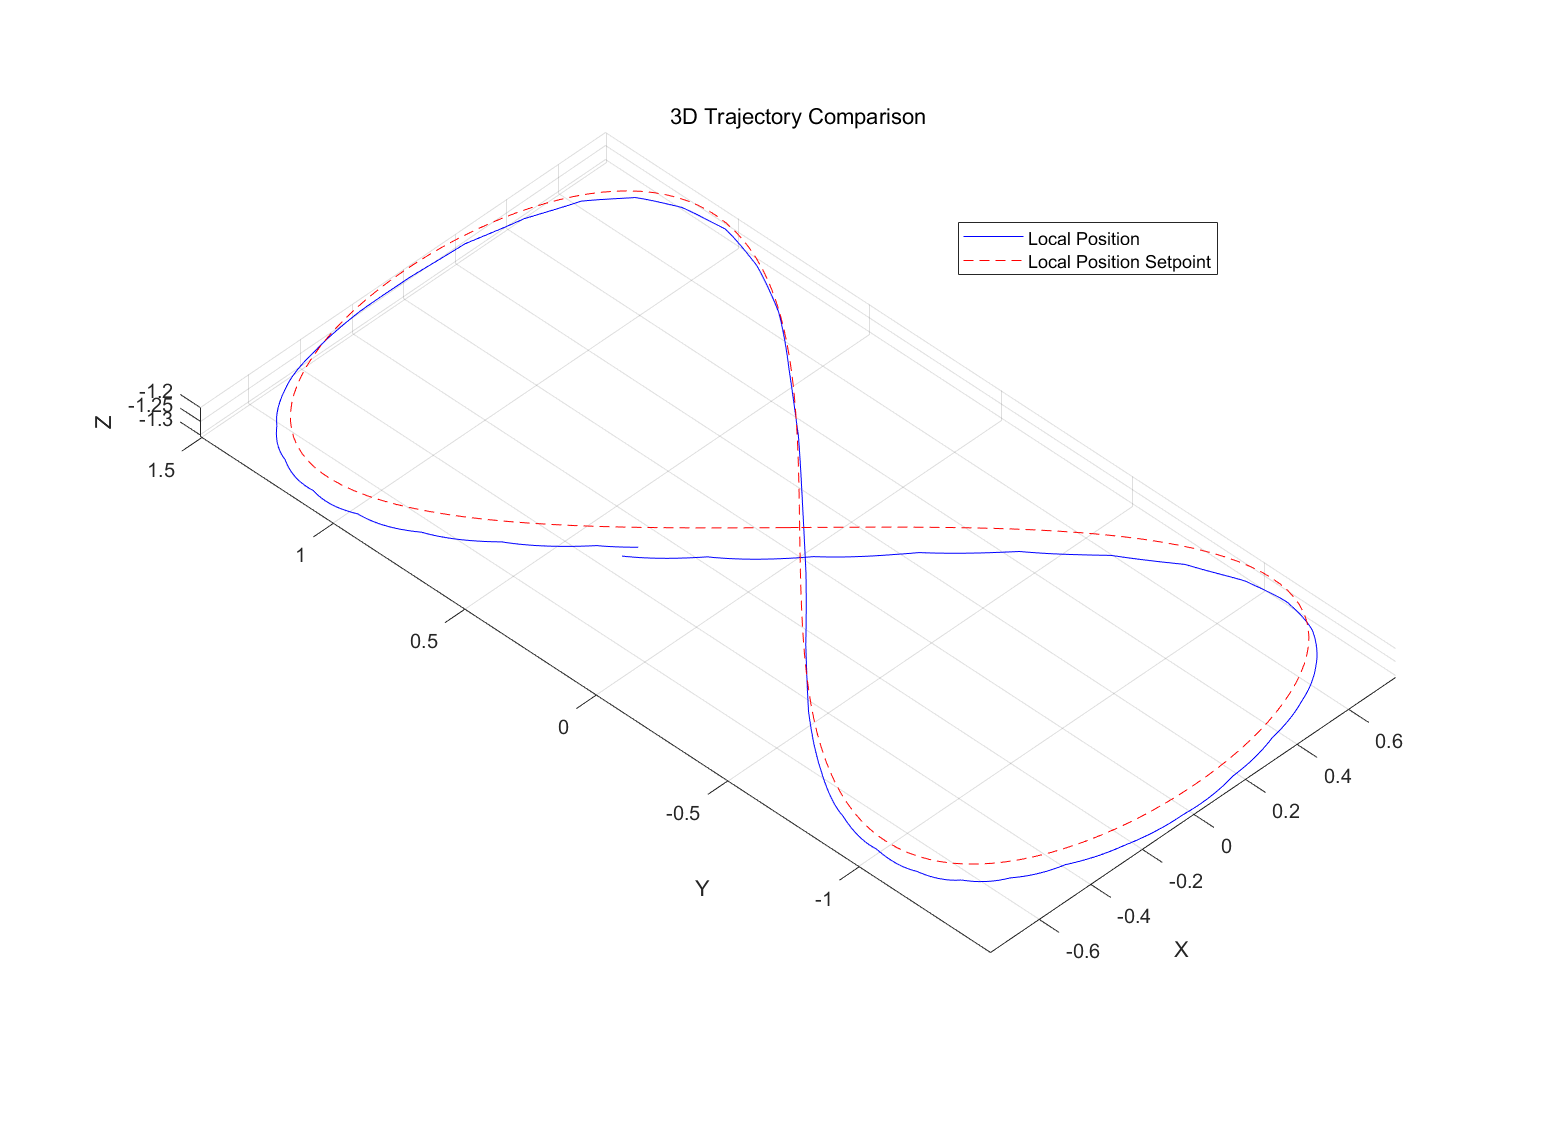
\includegraphics[width=\linewidth]{sitl_px4_3d.png}
      \caption{SITL下PX4三维轨迹跟踪效果}
  \end{minipage}
  \hfill % 在图片之间添加一些空间
  \begin{minipage}[b]{0.49\linewidth}
      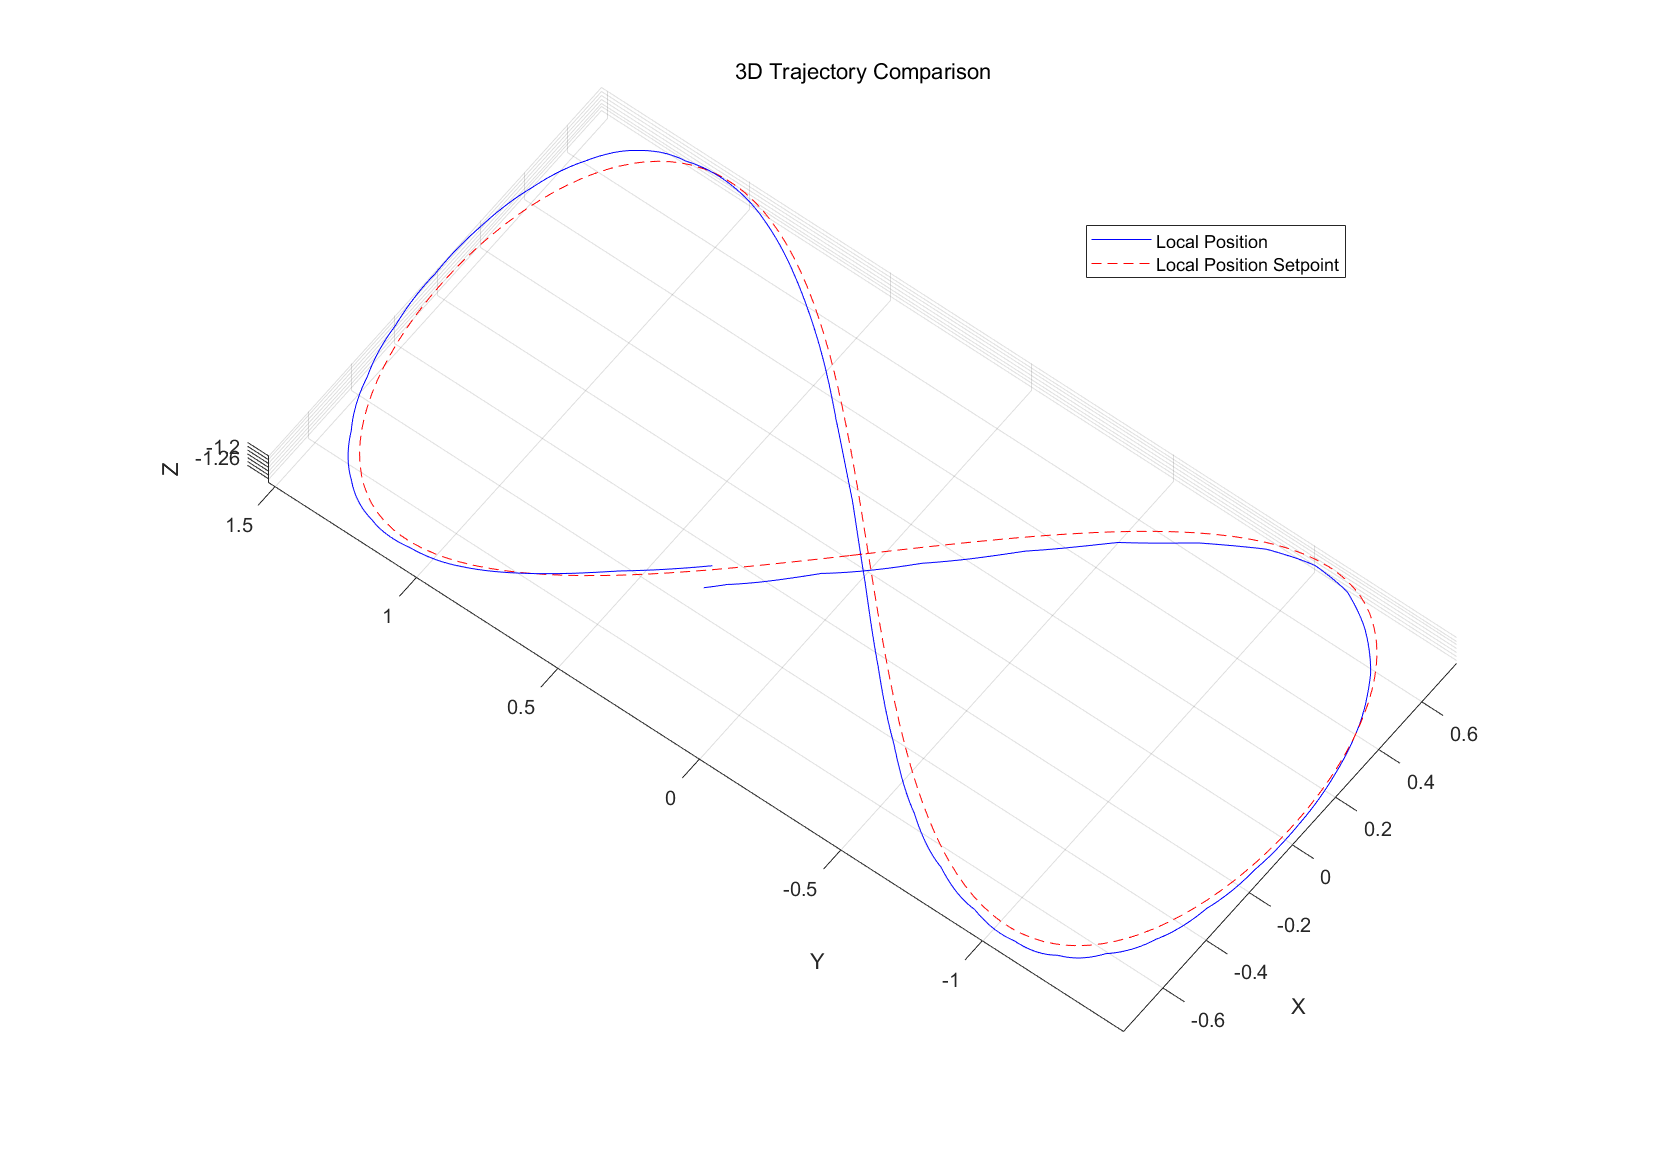
\includegraphics[width=\linewidth]{sitl_hofa_3d.png}
      \caption{SITL下HOFA三维轨迹跟踪效果}
  \end{minipage}

  %\vspace{1cm} % 在行之间添加一些垂直空间

  \begin{minipage}[b]{0.49\linewidth}
      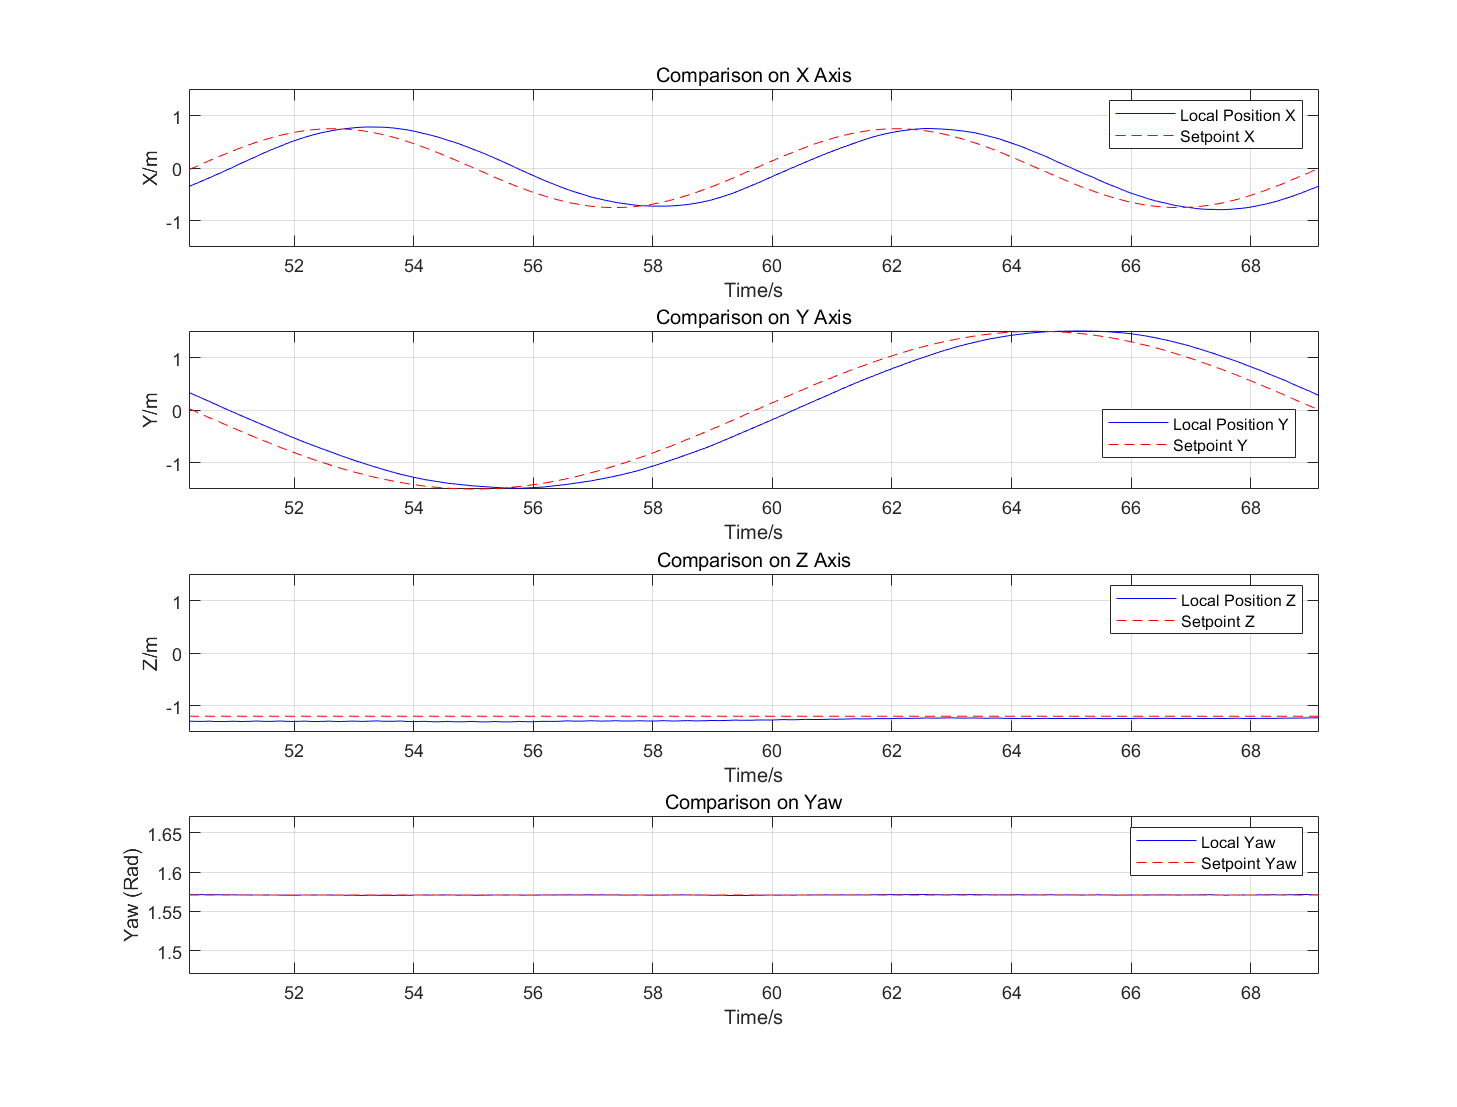
\includegraphics[width=\linewidth]{sitl_px4_xyzyaw.png}
      \caption{SITL下PX4各轴跟踪效果}
  \end{minipage}
  \hfill
  \begin{minipage}[b]{0.49\linewidth}
      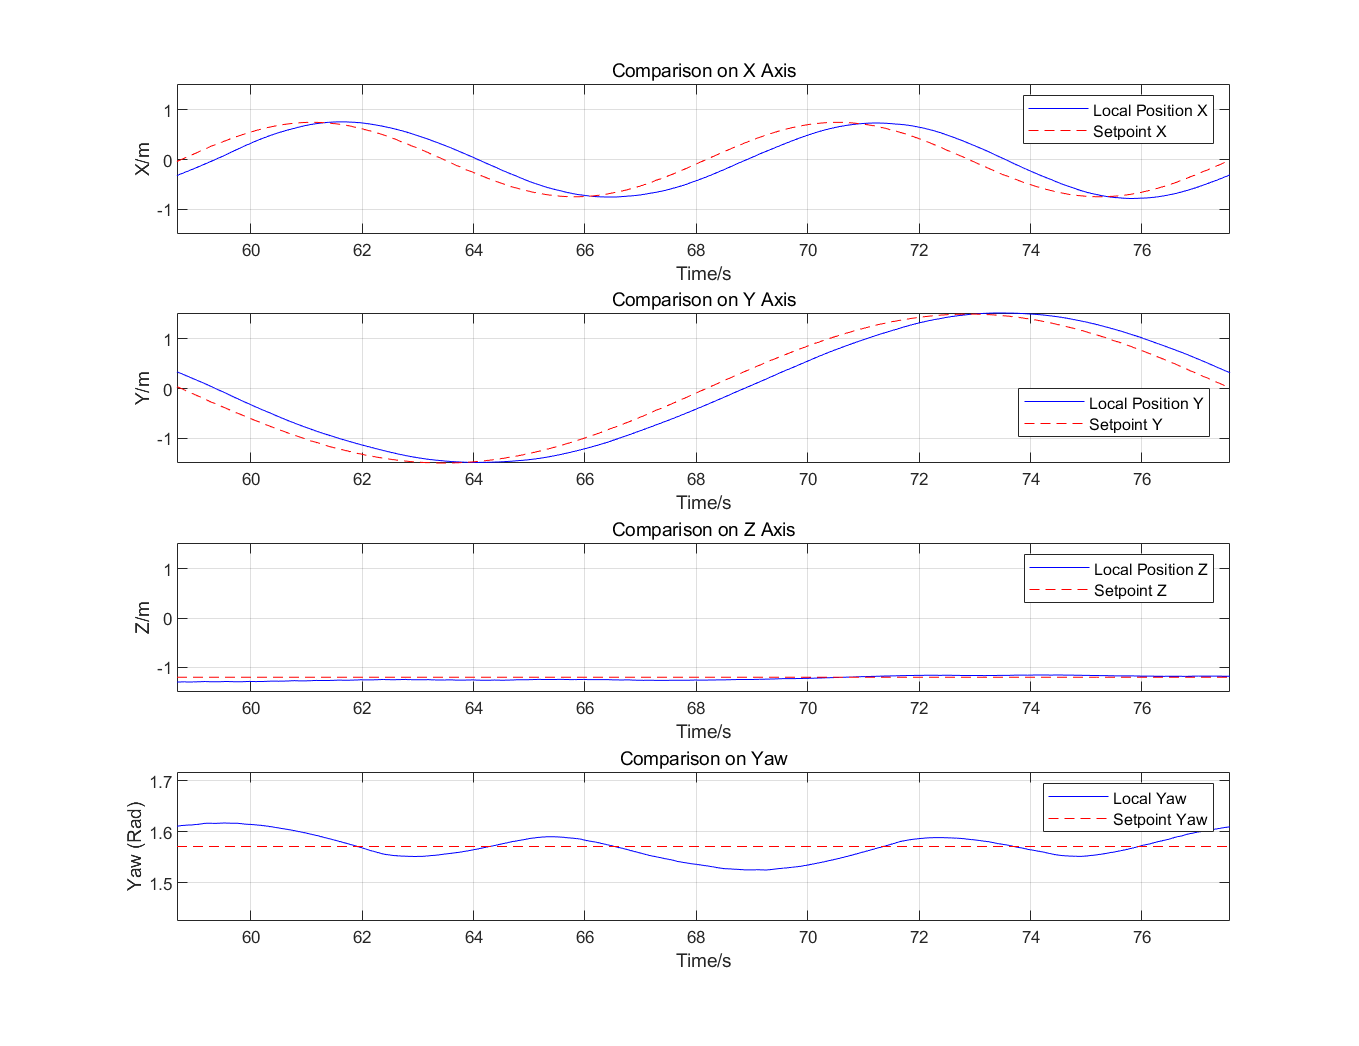
\includegraphics[width=\linewidth]{sitl_hofa_xyzyaw.png}
      \caption{SITL下HOFA各轴跟踪效果}
  \end{minipage}
\end{figure}

两者都能很好地跟踪“8”字型轨迹,对跟踪误差定量分析,计算每个时刻位置和期望位置的欧拉距离得到曲线如图\ref{sitl量化}、图\ref{sitl量化hofa}。

\begin{figure}[htb]
  \centering
  \begin{minipage}[b]{0.49\linewidth}
    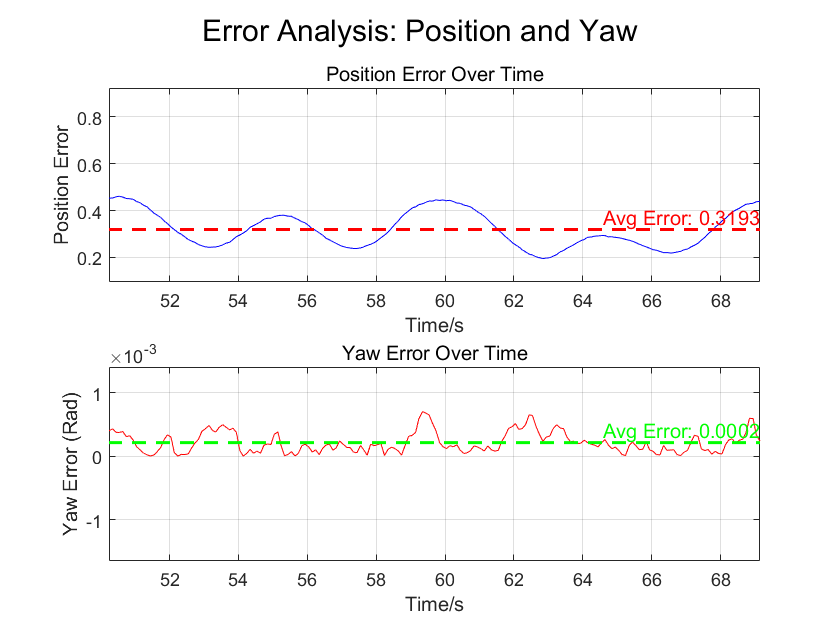
\includegraphics[width=\linewidth]{sitl_px4_e.png}
    \caption{SITL下PX4量化跟踪误差}
    \label{sitl量化}
\end{minipage}
\hfill
\begin{minipage}[b]{0.49\linewidth}
    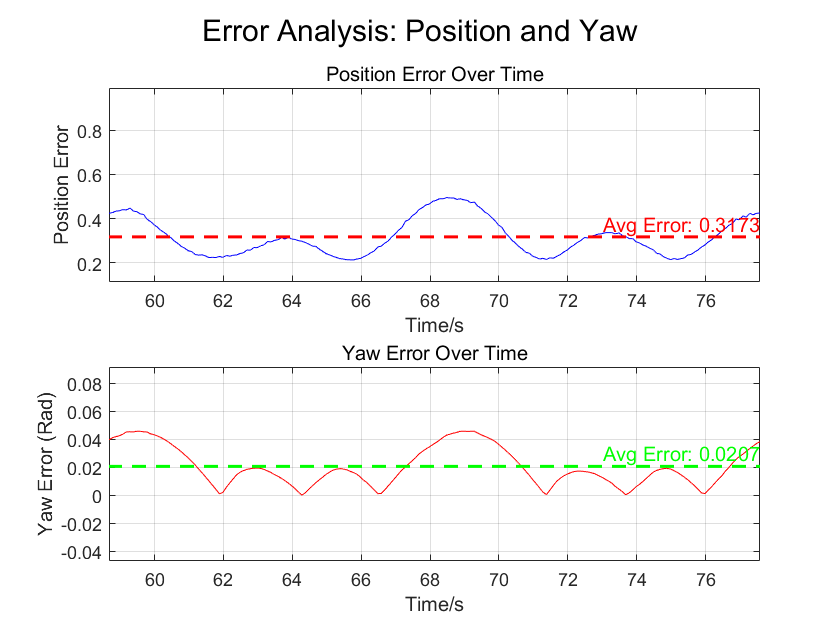
\includegraphics[width=\linewidth]{sitl_hofa_e.png}
    \caption{SITL下HOFA量化跟踪误差}
    \label{sitl量化hofa}
\end{minipage}

\end{figure}

从图\ref{sitl量化}、图\ref{sitl量化hofa}中标注的平均误差来看,在位置跟踪上HOFA略微优于PX4,两者的成绩都相当优秀,这从轨迹的形态上也可以看出。两者偏差都达到$0.32m$的原因在于偏差的计算方法是同一个时刻的位置和期望位置作差,而在速度不可以忽略的情况下,期望位置必然有相当的领先。在偏航角的控制上HOFA虽然不如PX4,但$0.0207 Rad$也是相当小的偏差。这是因为,在控制设计时就没有把偏航角作为主要的被控量,在LQR的参数选取上,偏航模态的权重要远小于滚转和俯仰。